%
% The first command in your LaTeX source must be the \documentclass command.
\documentclass[acmlarge,screen]{acmart}

%
% defining the \BibTeX command - from Oren Patashnik's original BibTeX documentation.
\def\BibTeX{{\rm B\kern-.05em{\sc i\kern-.025em b}\kern-.08emT\kern-.1667em\lower.7ex\hbox{E}\kern-.125emX}}

% Rights management information.
% This information is sent to you when you complete the rights form.
% These commands have SAMPLE values in them; it is your responsibility as an author to replace
% the commands and values with those provided to you when you complete the rights form.
%
% These commands are for a PROCEEDINGS abstract or paper.
\copyrightyear{2019}
\acmYear{2019}
\setcopyright{acmlicensed}
\acmConference[SIGGRAPH 2019]{SIGGRAPH 2019: THE 46TH INTERNATIONAL CONFERENCE & EXHIBITION ON COMPUTER GRAPHICS & INTERACTIVE TECHNIQUES}{28 July - 1 August, 2019}{Los Angeles, California}
\acmBooktitle{SIGGRAPH 2019: THE 46TH INTERNATIONAL CONFERENCE & EXHIBITION ON COMPUTER GRAPHICS & INTERACTIVE TECHNIQUES, 28 July - 1 August, 2019, Los Angeles, CA}
\acmPrice{15.00}
\acmDOI{10.1145/1122445.1122456}
\acmISBN{978-1-4503-9999-9/18/06}

%
% These commands are for a JOURNAL article.
%\setcopyright{acmcopyright}
%\acmJournal{TOG}
%\acmYear{2019}\acmVolume{37}\acmNumber{4}\acmArticle{111}\acmMonth{8}
%\acmDOI{10.1145/1122445.1122456}

%
% Submission ID.
% Use this when submitting an article to a sponsored event. You'll receive a unique submission ID from the organizers
% of the event, and this ID should be used as the parameter to this command.
%\acmSubmissionID{123-A56-BU3}

%
% The majority of ACM publications use numbered citations and references. If you are preparing content for an event
% sponsored by ACM SIGGRAPH, you must use the "author year" style of citations and references. Uncommenting
% the next command will enable that style.
%\citestyle{acmauthoryear}

%
% end of the preamble, start of the body of the document source.
\begin{document}

%
% The "title" command has an optional parameter, allowing the author to define a "short title" to be used in page headers.
\title{Reconstructing the MRI Aesthetic in Digital Holography}
\subtitle{A review of various techniques to identify the optimal approach for medical digital holograms}

%
% The "author" command and its associated commands are used to define the authors and their affiliations.
% Of note is the shared affiliation of the first two authors, and the "authornote" and "authornotemark" commands
% used to denote shared contribution to the research.
\author{Michael Page}
\email{mpage@faculty.ocadu.ca}
\orcid{1234-5678-9012}
\affiliation{%
  \institution{OCAD University}
  \streetaddress{205 Richmond Street West, Lower Level}
  \city{Toronto}
  \state{Ontario}
  \postcode{M5V 1V3}
}

\author{Jawa El Khash}
\email{jelkhash@faculty.ocadu.ca}
\orcid{1234-5678-9012}
\affiliation{%
  \institution{OCAD University}
  \streetaddress{205 Richmond Street West, Lower Level}
  \city{Toronto}
  \state{Ontario}
  \postcode{M5V 1V3}
}

\author{Adriana Menghi}
\email{amenghi@faculty.ocadu.ca}
\orcid{1234-5678-9012}
\affiliation{%
  \institution{OCAD University}
  \streetaddress{205 Richmond Street West, Lower Level}
  \city{Toronto}
  \state{Ontario}
  \postcode{M5V 1V3}
}

\author{Mario Garingo}
\email{mgaringo@ocadu.ca}
\orcid{1234-5678-9012}
\affiliation{%
  \institution{OCAD University}
  \streetaddress{205 Richmond Street West, Lower Level}
  \city{Toronto}
  \state{Ontario}
  \postcode{M5V 1V3}
}

\author{Marcus A. Gordon}
\email{mgordon@faculty.ocadu.ca}
\orcid{1234-5678-9012}
\affiliation{%
  \institution{OCAD University}
  \streetaddress{205 Richmond Street West, Lower Level}
  \city{Toronto}
  \state{Ontario}
  \postcode{M5V 1V3}
}

%
% By default, the full list of authors will be used in the page headers. Often, this list is too long, and will overlap
% other information printed in the page headers. This command allows the author to define a more concise list
% of authors' names for this purpose.
\renewcommand{\shortauthors}{Page and Gordon, et al.}

%
% The abstract is a short summary of the work to be presented in the article.
\begin{abstract}

In this research we propose a methodology that uses existing software tools to encode the MRI data into a multitude of two dimensional images. The proposed solution is the creation of a process that enables MRI data to be converted directly into a digital, holographic, print-ready form that requires no further processing and little to no human intervention.
\end{abstract}

%
% The code below is generated by the tool at http://dl.acm.org/ccs.cfm.
% Please copy and paste the code instead of the example below.
%
\begin{CCSXML}
<ccs2012>
<concept>
<concept_id>10010147.10010178.10010224.10010226.10010236</concept_id>
<concept_desc>Computing methodologies~Computational photography</concept_desc>
<concept_significance>500</concept_significance>
</concept>
<concept>
<concept_id>10010147.10010178.10010224.10010245.10010247</concept_id>
<concept_desc>Computing methodologies~Image segmentation</concept_desc>
<concept_significance>500</concept_significance>
</concept>
<concept>
<concept_id>10003456.10003462.10003602.10003608</concept_id>
<concept_desc>Social and professional topics~Medical technologies</concept_desc>
<concept_significance>500</concept_significance>
</concept>
<concept>
<concept_id>10010147.10010178.10010224.10010226.10010239</concept_id>
<concept_desc>Computing methodologies~3D imaging</concept_desc>
<concept_significance>500</concept_significance>
</concept>
<concept>
<concept_id>10010147.10010371.10010387.10010393</concept_id>
<concept_desc>Computing methodologies~Perception</concept_desc>
<concept_significance>300</concept_significance>
</concept>
<concept>
<concept_id>10010147.10010371.10010396.10010401</concept_id>
<concept_desc>Computing methodologies~Volumetric models</concept_desc>
<concept_significance>300</concept_significance>
</concept>
<concept>
<concept_id>10010147.10010371.10010372.10010374</concept_id>
<concept_desc>Computing methodologies~Ray tracing</concept_desc>
<concept_significance>100</concept_significance>
</concept>
<concept>
<concept_id>10010147.10010371.10010387.10010394</concept_id>
<concept_desc>Computing methodologies~Graphics file formats</concept_desc>
<concept_significance>500</concept_significance>
</concept>
<concept>
<concept_id>10010147.10010341.10010349.10010364</concept_id>
<concept_desc>Computing methodologies~Scientific visualization</concept_desc>
<concept_significance>300</concept_significance>
</concept>
<concept>
<concept_id>10010405.10010469.10010474</concept_id>
<concept_desc>Applied computing~Media arts</concept_desc>
<concept_significance>500</concept_significance>
</concept>
</ccs2012>
\end{CCSXML}

\ccsdesc[500]{Computing methodologies~Computational photography}
\ccsdesc[500]{Computing methodologies~Image segmentation}
\ccsdesc[500]{Social and professional topics~Medical technologies}
\ccsdesc[500]{Computing methodologies~3D imaging}
\ccsdesc[300]{Computing methodologies~Perception}
\ccsdesc[300]{Computing methodologies~Volumetric models}
\ccsdesc[100]{Computing methodologies~Ray tracing}
\ccsdesc[500]{Computing methodologies~Graphics file formats}
\ccsdesc[300]{Computing methodologies~Scientific visualization}
\ccsdesc[500]{Applied computing~Media arts}

%
% Keywords. The author(s) should pick words that accurately describe the work being
% presented. Separate the keywords with commas.
\keywords{digital holography, graphics pipeline, volume rendering, linear color, MRI}

%
% A "teaser" image appears between the author and affiliation information and the body
% of the document, and typically spans the page.
%%\begin{teaserfigure}
%%  \includegraphics[width=\textwidth]{sampleteaser}
%%  \caption{Seattle Mariners at Spring Training, 2010.}
%%  \Description{Enjoying the baseball game from the third-base seats. Ichiro Suzuki preparing to bat.}
%%  \label{fig:teaser}
%%\end{teaserfigure}

%
% This command processes the author and affiliation and title information and builds
% the first part of the formatted document.
\maketitle

\newpage
\section{Introduction}
\newpage
\subsection{}

\newpage
\section{Research Questions}
Is there a linear transformation that takes MRI images and creates holographic image stacks for printing?


\newpage
\section{Literature Review}
\input{sections/litReview/litReview.tex}

\newpage
\section{Methods}
In this section we will focus on the overall pipeline of the project as described in Figure \ref{fig:pipeline}.  This section will be divided into 4 sections: segmentation, generating 3D models or geometry, image stage generation, and finally digital holograms. 

\begin{figure}[H]
  \centering
  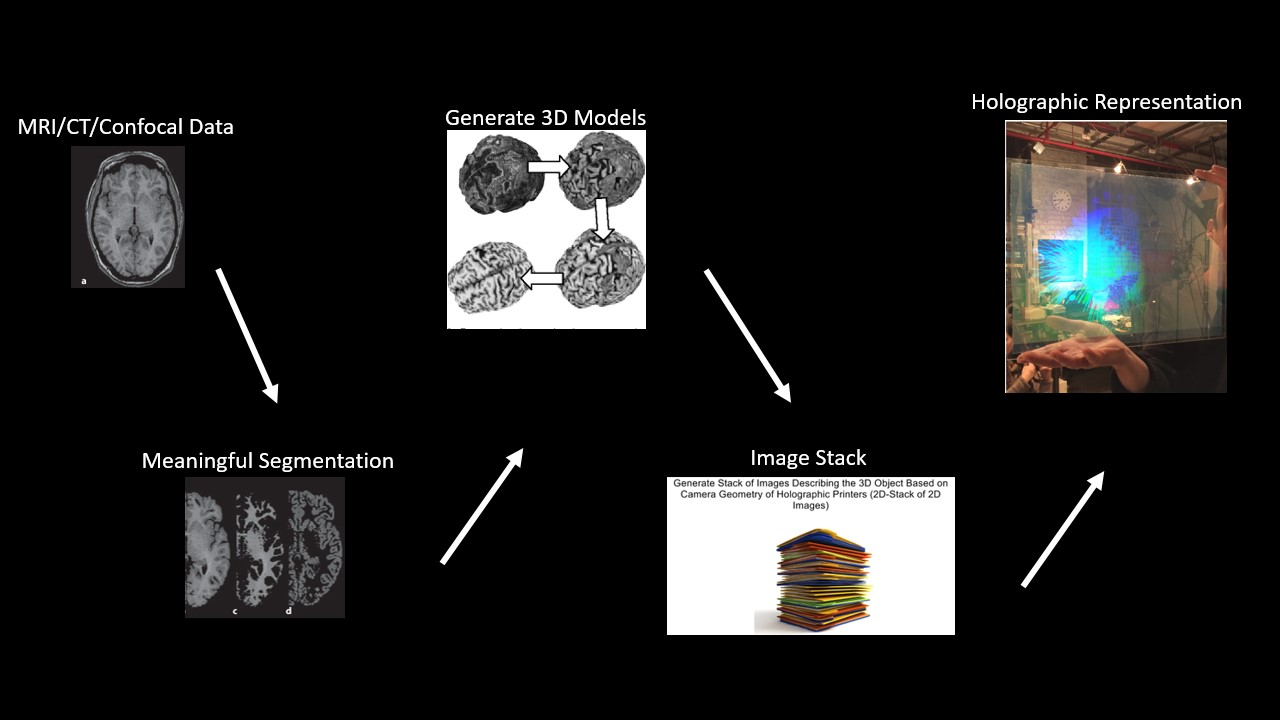
\includegraphics[width=\linewidth]{img/pipeline.jpg}
  \caption{General pipeline from medical image to a digital holographic print.}
  \label{fig:pipeline}
\end{figure}




\subsection{Segmentation}

The main objective of this project was to determine if the physicians/clinicians/technicians are able to obtain more meaningful information when given more depth information.  To give such information structural patterns within the model must be apparent. To achieve this we used a data-set of a human brain containing a tumor. The goal with the depth information inherently found in holography, the location of the tumor will become apparent.  As an intermediate step we need to develop geometry for each of the salient structures of the brain, mainly the white and gray matter, as well as the tumor and other abnormal tissues surrounding the tumor.  This is where segmentation algorithms are needed.\\

There are several different approaches that have been found throughout the literature \cite{pham2000current}.  But they all stem from the same set of core ideas.  Since the brain consists of known tissue types such as white and gray matter, bone and spinal fluid, the intuitive approach would be to classify these based on intensity values of the pixels on the MRI \cite{atkins1998fully}.  The problem arises when there are overlapping tissues and case intensity values of each pixel to be miss classified as one of the known tissue types \cite{undeman2003fully}.  This is why current MRI segmentation is not fully automated and radiologists are needed to help the computer identify which pixels are wrong and correct it. To combat this issue, there are some algorithms such as the one proposed by \cite{lenroot2006brain} whereby they use pre-segmented brain template and perform image registration and automatically identify the troublesome pixels and fix the labels accordingly.\\  

However necessary, the main purpose of this project is not on segmentation rather the depth information of the digital holographic print.  So we will not use complex and accurate segmentation techniques instead we will use the more intuitive approach of pixel classification using multithresholding (MT) techniques \cite{sahoo1988survey} in combination with region growing approaches\cite{adams1994seeded}.\\

The overall goal of MT is to generate masks which partition the image into our desired segmented areas.  To do this a histogram is first to identify the threshold ranges of each tissue type.  The segmentation is achieved by grouping similar pixel intensities together akin to quantizing the images.  But in this case the quantization levels are not constant. This is clearly seen in figure \ref{fig:mriHistogram}.  In the MRI you can see three distinct colours which corresponds to the white and gray matter (WM,GM) and also the cerebral fluid (CSF).  The histogram distributions show 3 distinct peak which corresponds to these tissue types.

\begin{figure}[H]
  \centering
  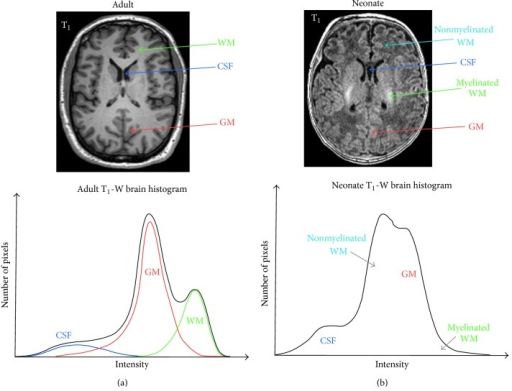
\includegraphics[width=\linewidth]{img/mriHistogram.png}
  \caption{MRI and pixel intensity histogram distribution.}
  \label{fig:mriHistogram}
\end{figure}

Notice the problem described earlier, there are overlapping pixels in the histogram that can be in either of the 3 labeled tissue classes.  We will combat this problem by introducing a region growing approach.\\

Region growing is a simple yet effective technique which samples and extracts a region of the image by connecting similar pixels together. Though very similar to thresholding, this introduces a fuzzy thresholding approach rather than categorical quantization.  The fuzzy approach comes about through the corporation of both the intenisty and edges of the image. The main step is to add a seed point which is manually selected, and from this point connect all the pixels surrounding it together and label that region accordingly.  In the literature this is often done for tumor and lesion segmentation\cite{guliato1998segmentation}. The main disadvantage of this approach is the resultant mask can be very noisy causing the extracted region to have holes and disconnected regions.  To remedy this affect we applied morphological filters\cite{mendiola2007morphological}. 
\subsection{Generating Geometry}

\subsubsection{Marching Cube Algorithm}

\subsubsection{Marcus Method}

\subsubsection{Jawa Method}
\subsection{Image Stack Generation}
\subsection{Digital Holograms}


\newpage
\section{Results}
Similarly to method section, this section will be divided into 4 main sections: segmentation, generating 3D models or geometry, image stage generation, and finally digital holograms. 






\newpage
\section{Discussion}

\newpage
\section{Conclusion and Future Work}

\newpage
\section{Bibliography}
\bibliography{sample-base.bib}
\bibliographystyle{acm}
\newpage

\end{document}
